\documentclass[12pt]{article}

\usepackage{fancyhdr}
\usepackage{makeidx}
\usepackage[catalan]{babel}
\usepackage{amsfonts}
\usepackage{amssymb}
\usepackage{amsthm}
\usepackage{amsmath}
\usepackage[all]{xy}
\usepackage[ansinew]{inputenc} %%
\usepackage[dvips]{epsfig}
\usepackage{color}



%\usepackage[spanish]{babel}
%\usepackage{color}% usar color para las letras
%\usepackage{graphics}
%\usepackage{graphicx}
%\usepackage{amssymb}
%\usepackage{amsfonts}%para poder poner las letras de Reales Complejos etc...
%\usepackage{anysize} % Soporte para el comando \marginsize
%\usepackage[latin1]{inputenc}% permite poner acentos de forma normal

\setlength{\textwidth}{16cm} \setlength{\textheight}{24cm}
\setlength{\oddsidemargin}{-0.3cm} \setlength{\topmargin}{-1.3cm}

%\usepackage{texfonts}
%\marginsize{2cm}{2cm}{2cm}{2cm}
%\newcommand{\ZZ}{\mathbbmss{Z}}
%\usepackage{fancyhdr}
%\renewcommand{\rmdefault}{phv}
%%%%%%%%%%%%%%%%%%%%%%%%%%%%%%%%%%%%%%%%%%%%%%%%%%%%%%%%%%%%%%%%%%%%%%%%
%-- nuevos comandos para facilitar la escritura
\newcommand{\notacio}{\textbf{Notaci{\'o}}\ \ }
\newcommand{\demostracio}{\textbf{Demostraci{\'o}}\ \ }
\newcommand{\propietats}{\textbf{Propietats}\ \ }
\newcommand{\propietat}{\textbf{Propietat}\ \ }
%\newcommand{\exemple}{\textbf{Exemple}\ \ }
\newcommand{\exemples}{\textbf{Exemples}\ \ }
\newcommand{\observacio}{\textbf{Observaci{\'o}}\ \ }
\newcommand{\observacions}{\textbf{Observacions}\ \ }
\newcommand{\solucio}{\textbf{Soluci{\'o}}\ \ }


\newtheorem{definicio}{Definici{\'o}}[subsection]
\newtheorem{teorema}{Teorema}[subsection]
\newtheorem{Teorema}{Teorema}[subsubsection]
\newtheorem{proposicio}{Proposici{\'o}}[subsection]
\newtheorem{lema}{Lema}[subsection]
\newtheorem{corol}{Corol.lari}[subsection]
\newtheorem{exemple}{Exemple}[subsection]
\newtheorem{prob}{Problema}[subsection]


\newcommand{\Z}{\mathbb{Z}}
\newcommand{\R}{\mathbb{R}}
\newcommand{\C}{\mathbb{C}}
\newcommand{\N}{\mathbb{N}}
\newcommand{\U}{\mathcal{U}}
\newcommand{\V}{\mathcal{V}}
\newcommand{\W}{\mathcal{W}}
\newcommand{\sen}{\mathop{\rm sen}\nolimits}

\setcounter{page}{10}

\setcounter{section}{1}

\begin{document}

\parskip =0.3cm
\parindent =0cm
\itemindent=2cm


\begin{center}
%\section{Introducci{\'o} als espais euclidians i normats}
\section{L{\'\i}mits i continu{\"\i}tat}
\end{center}


\vspace*{0.7cm}
\subsection{Introducci{\'o} a les funcions de diverses variables}

Sovint en el m{\'o}n real, el valor d'una quantitat no dep{\`e}n nom{\'e}s d'una variable.
Sin{\'o} de dues o m{\'e}s variables. Per exemple:
\begin{itemize}
\item[-] Suposem que tenim una l{\`a}mina met{\`a}l.lica i ens interessa estudiar la temperatura
en diversos punts de la l{\`a}mina a l'instant $t$. Si representam els punts de la l{\`a}mina per
parells $(x,y)$ de nombres reals, llavors la temperatura $T$ es pot expressar com una
funci{\'o} de dues variables de localitzaci{\'o} $x,\, y$ i d'una variable temporal $t$ (temps).

Aix{\'\i}, la temperatura $T$ dep{\`e}n, en aquest cas, de tres variables i ho escrivim de la
forma $T(x,y,t)$.
\end{itemize}

Per tant {\'e}s interessant considerar funcions
$f\, :\, \R^n \longrightarrow \R^m$ amb $n$ i $m$ finits i naturals no nuls i, el nostre
inter{\`e}s es centrar{\`a} en estendre els conceptes de l{\'\i}mit, continu{\"\i}tat, derivabilitat i integraci{\'o} que ja coneixem per funcions reals de variable real a funcions de diverses variables.

Comen\c{c}arem donant els conceptes b{\`a}sics com s{\'o}n: domini i
rang, gr{\`a}fica i corbes de nivell d'una funci{\'o} de dues
variables i despr{\'e}s generalitzarem a funcions de 3 i m{\'e}s
variables.

\subsection{Conceptes b{\`a}sics}

\begin{definicio}[Funci{\'o} real de dues variables reals]
Sigui $D\subset \R^2$. Una \textbf{funci{\'o} de dues variables} {\'e}s una
regla que assigna a cada parell $(x,y)\in D$ un {\'u}nic nombre
real denotat per $f(x,y)$.
\end{definicio}

Ho escriurem com
\begin{align*}
f\, :\, D\subset\R^2 & \longrightarrow \R \\ (x,y) & \mapsto
f(x,y)
\end{align*}
El conjunt $D$ s'anomena \textbf{domini} de $f$ i el \textbf{rang} de $f$ {\'e}s el
conjunt format pels valors de $f(x,y)$ quan $(x,y)\in D$.
\[
\mbox{rang}(f)=\{f(x,y)\, : \, (x,y)\in D \}
\]
Sovint denotarem una funci{\'o} de dues variables per $z=f(x,y)$ on
$x,\, y$ direm que s{\'o}n les variables independents i $z$ la
variable dependent.



\vspace{0.4cm}
\observacio
Si una funci{\'o} $f$ ve donada per una f{\'o}rmula sense especificar
el seu domini, aleshores el domini $D$ de $f$ ve donat pel conjunt
de parells $(x,y)\in D$ pels quals l'expressi{\'o} donada defineix
un n{\'u}mero real.


Habitualment una funci{\'o} $f\, :\, \R^2\longrightarrow \R$ no
estar{\`a} definida en tot $\R^2$, com per exemple
\[
f(x,y)=\sin \left( \frac{1}{x+y}\right)
\]
que no existeix on $x+y=0$.


\vspace{0.4cm}
\begin{exemple}
Sigui $f(x,y)=\sqrt{1-x+y}$. Avaluau $f(2,1)$, $f(-4,3)$ i trobau
el seu domini.
\end{exemple}

\solucio
Tenim que

$
  f(2,1)  =  \sqrt{1-2+1}=0\qquad \qquad f(-4,3) = \sqrt{1+4+3}=\sqrt{8}=2\sqrt{2}$

El seu domini ve donat per
\begin{align*}
  D & = \{ (x,y)\in \R^2\, :\, \sqrt{1-x+y}\in \R \} = \{ (x,y)\in \R^2\, :\, 1-x+y\geq 0 \} \\
  &\\
   & =\{ (x,y)\in \R^2\, :\, y\geq x-1 \}
\end{align*}

En la figura \ref{fig1} podeu veure la seva representaci{\'o} gr{\`a}fica.

\begin{figure}[h!]
\begin{center}
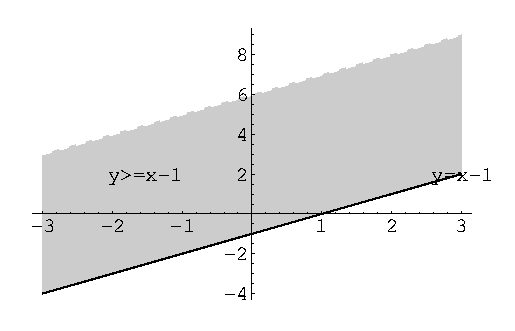
\epsfig{file=Graf1.eps,clip=}
\vspace{-.4cm}
\end{center}
\caption{Domini de la funci{\'o} $f(x)=\sqrt{1-x+y}$}\label{fig1}
\end{figure}


\vspace{0.7cm}
\begin{exemple}
Sigui $f(x,y)=\frac{\sqrt{x+y+1}}{x-1}$. Avaluau $f(3,2)$ i trobau
el seu domini.
\end{exemple}

\solucio
\[
f(3,2)=\frac{\sqrt{3+2+1}}{3-1} = \frac{\sqrt{6}}{2}
\]

El domini est{\`a} format pels punts $(x,y)\in \R^2$ tals que

\[
\frac{\sqrt{x+y+1}}{x-1}\in\R^2 \; \Longleftrightarrow \;
x+y+1\geq 0\,\; \mbox{i}\,\; x-1\not= 0.
\]

\vspace{0.4cm}
Per tant $D=\{(x,y)\in\R\, :\, y\geq -x-1  \quad \mbox{i}\quad
x\not= 1\}$

Si el representam gr{\`a}ficament el domini est{\`a} format pel
semipl{\`a} que queda per damunt la recta $y=-x-1$ llevat dels punts
que estan sobre la recta $x=1$.
\begin{figure}[h!]
\begin{center}
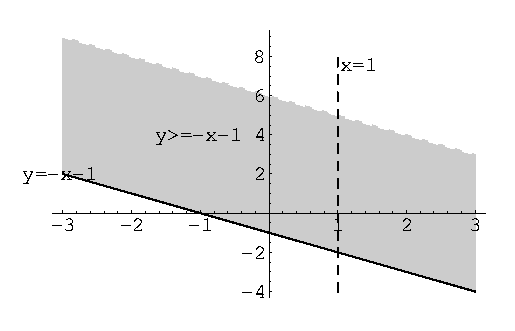
\epsfig{file=Graf2.eps,clip=}
\vspace{-.4cm}
\end{center}
\caption{Domini de la funci{\'o} $f(x)=\frac{\sqrt{x+y+1}}{x-1}$}
\end{figure}

%\vspace{0.4cm}
%\begin{exemple}
%Sigui $f(x,y)=x\ln (y^2 -x)$. Trobau el seu domini i avaluau
%$f(3,2)$.
%\end{exemple}
%
%\solucio
%Tenim que
%\[
%  f(3,2) = 3\ln (4-3)= 3\ln 1 = 0
%\]
%El seu domini ve donat per
%
%$$
%  D  = \{ (x,y)\in \R^2\ :\ y^2 -x > 0 \} =\{ (x,y)\in \R^2\ :\ x< y^2 \}
%$$
%
%%Gr{\`a}ficament podem veure el domini en la Figura \ref{ejemploFDV3}.
%\begin{figure}[h!]
%\begin{center}
%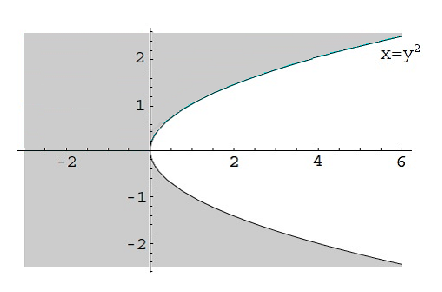
\epsfig{file=Graf3.eps,clip=}
%\end{center}
%\caption{Domini de la funci{\'o} $f(x)=x\ln (y^2 -x)$}\label{ejemploFDV3}
%\end{figure}

\vspace{0.4cm}
\begin{definicio}[Gr{\`a}fica d'una funci{\'o} de dues variables]
Si $f$ {\'e}s una funci{\'o} de dues variables amb domini $D$, \textbf{la
gr{\`a}fica de $f$} {\'e}s el conjunt
\[
S=G(f)=\{(x,y,z)\in \R^3\, :\, z=f(x,y),\; (x,y)\in D  \}.
\]
\end{definicio}

De la definici{\'o} observam que la gr{\`a}fica {\'e}s una superf{\'\i}cie en $\R^3$
d'equaci{\'o} $z=f(x,y)$. La seva projecci{\'o} sobre el pla
$xy$ {\'e}s el domini $D$ (vegeu la Figura \ref{projeccioFDV}).

\begin{figure}[h!]
\begin{center}
\input{figProyD.pstex_t}
\vspace{-.4cm}
\end{center}\caption{Projecci{\'o} d'una funci{\'o} real de dues variables reals}\label{projeccioFDV}
\end{figure}


A difer{\`e}ncia de funcions d'una variable, dibuixar la gr{\`a}fica d'una funci{\'o} de dues
variables {\'e}s bastant m{\'e}s complicat, a m{\'e}s quan la funci{\'o} {\'e}s de m{\'e}s de dues
variables (o b{\'e} una funci{\'o} vectorial) la representaci{\'o} gr{\`a}fica {\'e}s impossible.

\vspace*{0.4cm}
\begin{exemple}
Dibuixau la gr{\`a}fica de la funci{\'o} $f(x,y)=6-3x-2y$.
\end{exemple}

\solucio
La gr{\`a}fica de $f$ ve donada per l'equaci{\'o} $z=6-3x-2y$, {\'e}s a
dir, $3x+2y+z=6$, que no {\'e}s m{\'e}s que l'equaci{\'o} d'un pla. \'Es
el pla que passa pels punts $(2,0,0)$, $(0,3,0)$ i $(0,0,6)$.



\vspace*{0.4cm}
\begin{exemple}
Sigui $\ g(x,y)=\sqrt{9-x^2-y^2}$. Calculau el domini, el rang i dibuixau
la gr{\`a}fica de $g$.
\end{exemple}

\vspace{0.4 cm}
\solucio
\[
  D = \{(x,y)\in \R^2\ :\ 9-x^2-y^2\geq 0
  \},
\]
per{\`o}, $\ 9-x^2-y^2\geq 0\ $ si, i nom{\'e}s si, $\ x^2+y^2 \leq 9\ $ i,
per tant, el domini {\'e}s el disc de centre $(0,0)$ i radi 3.\\

Per altra part
\[
\mbox{rang}(g)=\{z\in\R\ :\ z=\sqrt{9-x^2-y^2},\; (x,y)\in D
\}
\]
$z$ {\'e}s una arrel quadrada positiva, per tant, $z\geq 0$.

\noindent Per altra banda
\[
9-x^2 - y^2 \leq 9 \ \Longrightarrow\ \sqrt{9-x^2-y^2}\leq 3
\]
aix{\'\i}
\[
\mbox{rang}(g)= \{z\in\R\,\; :\,\; 0\leq z\leq 3   \}=[ 0,3 ]
\]

La gr{\`a}fica ve donada per l'equaci{\'o}
\[
 z=\sqrt{9-x^2-y^2}
\]
si elevam al quadrat ambd{\'o}s membres de l'equaci{\'o} resulta
\[
z^2 = 9-x^2-y^2\,\; \Longleftrightarrow\,\; x^2+y^2+z^2=9
\]


que {\'e}s l'equaci{\'o} d'una esfera de centre l'origen $(0,0,0)$ i
radi 3. Per{\`o} com que $z\geq 0$, la gr{\`a}fica {\'e}s la semiesfera
superior.
\begin{figure}[h!]
\begin{center}
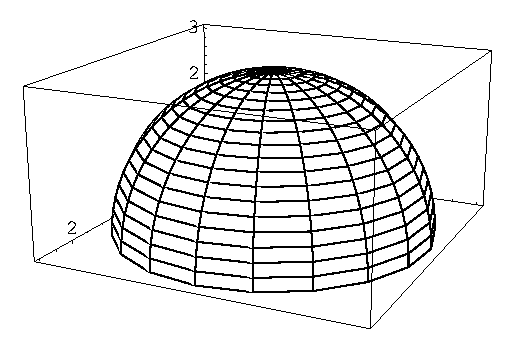
\epsfig{file=Graf5.eps,clip=}
\vspace{-.8cm}
\end{center}\caption{Gr{\`a}fica de  $\ g(x,y)=\sqrt{9-x^2-y^2}$.}
\end{figure}


\vspace{1cm}
Un m{\`e}tode {\'u}til per estudiar la
gr{\`a}fica d'una funci{\'o} real de dues variables reals {\'e}s fent
{\'u}s de les nomenades corbes de nivell.

\begin{definicio}
Sigui $\ f:D\subset \R^2\longrightarrow \R\,.$ El conjunt de
punts del pla $xy$ que satisfan l'equaci{\'o} $f(x,y)=k$, s'anomena
\textbf{corba de nivell} $k$, on $k$ {\'e}s constant i $k\in\mbox{rang}(f)$.
\end{definicio}



Per exemple, suposem que la superf{\'\i}cie $z=f(x,y)$ {\'e}s una
muntanya. Si volem dibuixar un mapa bidimensional de la muntanya, podem dibuixar en el pla les corbes d'altura constant, indicant amb
una etiqueta aquesta altura, obtenint aix{\'\i} un mapa
topogr{\`a}fic de la superf{\'\i}cie $z=f(x,y)$.

Altres exemples de corbes de nivell s{\'o}n les que apareixen en els
mapes de predicci{\'o} metereol{\`o}gica. Les corbes corresponents als
punts amb la mateixa temperatura s{\'o}n les isotermes i les
corresponents als punts amb la mateixa pressi{\'o} atmosf{\`e}rica
s{\'o}n les is{\`o}bares.

\vspace*{0.4 cm}
\begin{exemple}
Dibuixau les corbes de nivell de les funcions seg{\"u}ents per als
valors de $k$ indicats.
\end{exemple}

\solucio
\begin{itemize}
\item[1.-] $f(x,y)=6-3x-2y\,,\qquad k=-6,0,6$.

  \[
6-3x-2y=k\ \Longrightarrow\  3x+2y+k-6=0
  \]
  {\'e}s l'equaci{\'o} d'una fam{\'\i}lia de rectes amb pendent
  $-\frac{3}{2}$.

\begin{align*}
  & k=-6 & 3x+2y-12=0, \\
  & k=0 & 3x+2y-6=0,\\
  & k=6 & 3x+2y=0.
\end{align*}
\begin{figure}[h!]
\begin{center}
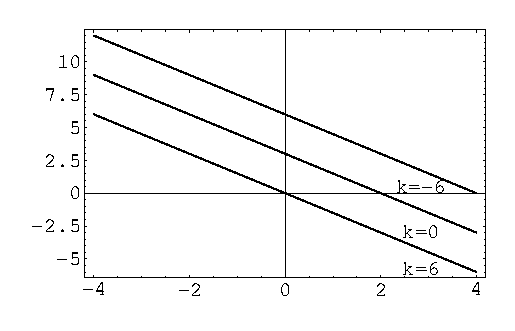
\epsfig{file=Graf7.eps,clip=,width=6cm,height=4cm}
\vspace{-.4cm}
\end{center}\caption{Corbes de nivell de la funci{\'o}  $f(x,y)=6-3x-2y$}
\end{figure}

%  \item[2.-] $f(x,y)=x y\,,\qquad k=1,2$.
%
%  \[
%  f(x,y)=xy\,\; \Longrightarrow\,\; y=\frac{k}{x}
%  \]
%  {\'e}s l'equaci{\'o} d'una fam{\'\i}lia d'hip{\`e}rboles.
%
%\begin{figure}[h!]
%\begin{center}
%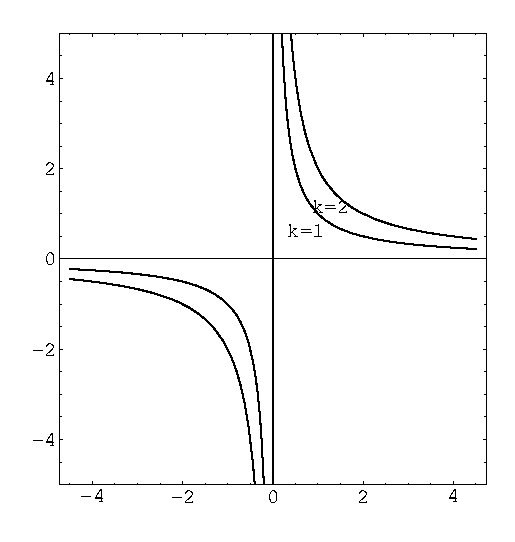
\epsfig{file=Graf8.eps,clip=,width=6cm,height=6cm}
%\vspace{-.4cm}
%\end{center}\caption{Corbes de nivell de la funci{\'o}  $f(x,y)=xy$}
%\end{figure}

%\vspace*{0.3 cm}
%\item[2.-] $f(x,y)=\sqrt{9-x^2-y^2}\,,\qquad k=0,1,3$.
%
%\[
%\sqrt{9-x^2-y^2}=k\,\; \Longleftrightarrow\,\; 9-x^2-y^2=k^2\,\;
%\Longleftrightarrow\,\; x^2+y^2=9-k^2
%\]
%
%circumfer{\`e}ncies de centre $\ (0,0)\ $ i radi $\ r=\sqrt{9-k^2}$.
%\begin{align*}
%  &k=0 & r=3 \\
%  &k=1 & r=2\sqrt{2} \\
%  &k=3 & r=0\,\; \Longrightarrow\,\; \mbox{\'Es el punt}\,\; (0,0).
%\end{align*}
%\vskip -0.5 cm
%\begin{figure}[h!]
%\begin{center}
%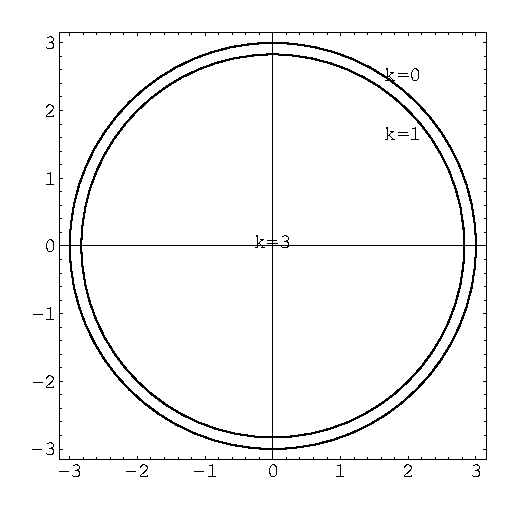
\epsfig{file=Graf9.eps,clip=,width=4cm,height=4cm}
%\vspace{-.4cm}
%\end{center}\caption{Corbes de nivell de la funci{\'o}  $f(x,y)=\sqrt{9-x^2-y^2}$}
%\end{figure}

%\vspace*{0.3 cm}
%\item[4.-]  $f(x,y)=x+y^2\,,\qquad k=0,2$.
%  \[
%x+y^2=k\,\; \Longrightarrow\,\; x= - y^2 + k
%  \]
%  que {\'e}s una fam{\'\i}lia de par{\`a}boles.
%\begin{align*}
%  &k=0 & x=-y^2, \\
% &k=2 & x=-y^2+2.
% \end{align*}
%\begin{figure}[h!]
%\begin{center}
%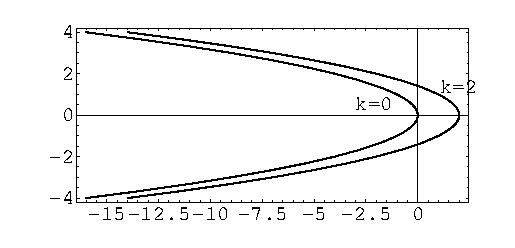
\epsfig{file=Graf11.eps,clip=}
%\vspace{-.4cm}
%\end{center}\caption{Corbes de nivell de la funci{\'o} $f(x,y)=x+y^2$}
%\end{figure}
%
%A partir d'aix{\`o} podem representar la gr{\`a}fica de la funci{\'o}:
%\begin{figure}[h!]
%\begin{center}
%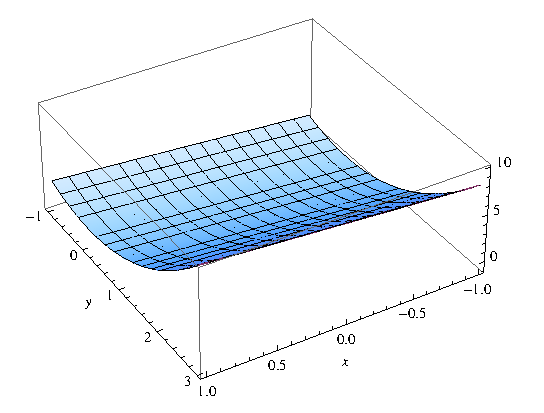
\epsfig{file=Graf12.eps,clip=}
%\vspace{-.4cm}
%\end{center}\caption{Representaci{\'o} gr{\`a}fica de la funci{\'o}  $f(x,y)=x+y^2$}
%\end{figure}



\vspace*{0.3 cm}
  \item[2.-] $f(x,y)=4x^2+y^2\,,\qquad k=1,4$.\\

Tenim que $\
4x^2+y^2=k\,\; \Longleftrightarrow\,\; \frac{4x^2}{k} +
\frac{y^2}{k}=1\,\; \Longleftrightarrow\,\;
\frac{x^2}{\frac{k}{4}} + \frac{y^2}{k}=1,
  $
  que {\'e}s la fam{\'\i}lia d'el.lipses de semieixos $\frac{\sqrt{k}}{2}$ i
  $\sqrt{k}$ i centrades a l'origen $(0,0)$.

%begin{align*}
%  &k=1 & \frac{x^2}{1/4} + \frac{y^2}{1}=1, \\
%  &\\
% &k=4 & \frac{x^2}{1} + \frac{y^2}{4}=1.
% \end{align*}
\begin{figure}[h!]
\begin{center}
%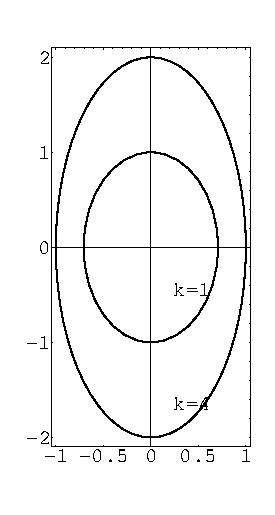
\epsfig{file=Graf10.eps,clip=}
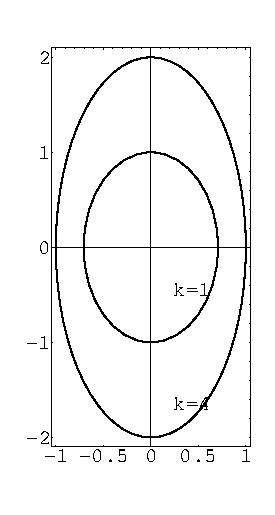
\includegraphics[width=2.5cm]{Graf10.eps}
\vspace{-.6cm}
\end{center}\caption{Corbes de nivell de la funci{\'o}  $f(x,y)=4x^2+y^2$}
\end{figure}


L'equaci{\'o} de la gr{\`a}fica de $f$ ve donada per $z=4x^2 + y^2$ que resulta
l'equaci{\'o} d'un paraboloide el.l{\'\i}ptic. (Veure la figura \ref{paraboloide}).\\

Aquesta superf{\'\i}cie {\'e}s una paraboloide ja que si fixam $x=k$ obtenim  $\ z=y^2+4k^2\ $ que {\'e}s una par{\`a}bola en el pla $yz$ i si fixam $y=c$ obtenim  $\ z=4x^2+c^2\ $ que {\'e}s una par{\`a}bola en el pla $xz$.
\begin{figure}[h!]
\begin{center}
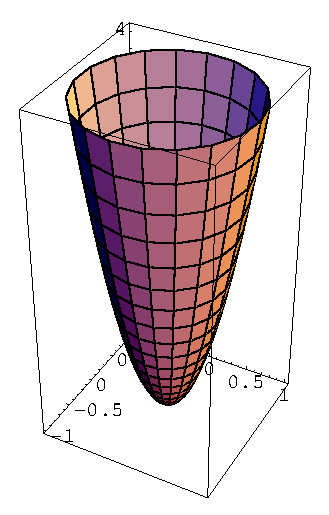
\epsfig{file=Graf6.eps,clip=,height=4cm,width=3cm}
\end{center}\caption{Gr{\`a}fica de  $\ \ f(x,y)= 4x^2 + y^2$.}\label{paraboloide}
\end{figure}
\end{itemize}


\vspace{1cm}
\begin{definicio}[Funci{\'o} real de tres variables reals]
Sigui $D\subset \R^3$. Una \textbf{funci{\'o} real de tres variables}, $f$, {\'e}s
una regla que assigna a cada terna ordenada $(x,y,z)$ del domini $
D$ un {\'u}nic n{\'u}mero real denotat per $f(x,y,z)$.
\end{definicio}

%\vspace{0.4cm}
%\begin{exemple}
%Donada la funci{\'o} $f(x,y,z)=\ln (z-y) + xy\sin z$ el seu domini
%{\'e}s
%\[
%D=\{(x,y,z)\in\R^3\,\; : \,\; z-y> 0  \}.
%\]
%{\'E}s el semiespai format pels punts que estan per damunt del pla
%$z=y$.
%\end{exemple}

{\'E}s clar que no podem dibuixar la gr{\`a}fica d'una funci{\'o} de
tres variables ja que seria necessari un espai de dimensi{\'o} 4.
Per poder intuir el comportament d'una funci{\'o} de tres variables,
es poden estudiar les nomenades superf{\'\i}cies de nivell.

\vspace{0.4cm}
\begin{definicio}
Si $k\in \mbox{rang}(f)$, $k$ constant, s'anomena \textbf{superf{\'\i}cie
de nivell} $k$ a la superf{\'\i}cie de $\R^3$ definida per
$f(x,y,z)=k$.
\end{definicio}

%\vspace{0.4cm}
%\begin{exemple}
%Trobau les superf{\'\i}cies de nivell de la funci{\'o}
%  $f(x,y,z)=x^2+y^2+z^2$.
%\end{exemple}
%
%
%\solucio
%  $x^2+y^2+z^2=k$, amb $k\geq 0$ {\'e}s la fam{\'\i}lia d'esferes
%  amb centre $(0,0,0)$ i radi $\sqrt{k}$.

\vspace{0.4cm}
\begin{exemple}
Suposem que la temperatura $T$ en cada punt $(x,y,z)$
  d'una regi{\'o} $R$, ve donada per $T(x,y,z)=100-x^2-y^2-z^2$  graus celsius.
  Descriviu les superf{\'\i}cies isotermes per a $T > 0$.
\end{exemple}

\solucio
  $T(x,y,z)=k$, amb $k> 0$ obtenim $100-x^2-y^2-z^2 = k$,
  aleshores $x^2+y^2+z^2=100-k$.

  \noindent Si $100-k > 0$ obtenim la fam{\'\i}lia d'esferes amb
  centre l'origen de coordenades i $r=\sqrt{100-k}$.

  \noindent Si $100-k=0$, aleshores $k=100$ i obtenim l'origen de
  coordenades.

\vspace{0.4cm}
\begin{definicio}[Funci{\'o} real de $n$ variables reals]
Sigui $D\subset \R^n$. Una \textbf{funci{\'o} real de $n$ variables} {\'e}s una
regla que assigna a cada n-pla $(x_1,x_2,\ldots ,x_n)$ del conjunt
$D$ un {\'u}nic n{\'u}mero real denotat per $f(x_1,x_2,\ldots ,x_n)$.
\end{definicio}


\hspace{3cm}
$
\begin{array}{cccc}
f\, :& D\subset \R^n\, & \longrightarrow & \,\R \\
&(x_1,x_2,\ldots ,x_n) &\longrightarrow & f(x_1,x_2,\ldots ,x_n)
\end{array}
$

\vspace{0.2cm}
El conjunt $D$ s'anomena \textbf{domini} de $f$ i el \textbf{rang} de $f$ {\'e}s el
conjunt format pels valors de $f(x_1,x_2,\ldots ,x_n)$ quan
$(x_1,x_2,\ldots ,x_n)\in D$,
\[
\mbox{rang}(f)=\{f(x_1,x_2,\ldots ,x_n)\in\R\, :\, (x_1,x_2,\ldots
,x_n)\in D  \} .
\]

De la mateixa manera definim el \textbf{graf} d'una
funci{\'o} $f\, :\, D\subset \R^n\,  \longrightarrow \,\R$ com el
conjunt de punts
\[
S=G(f)=\{ (x_1,x_2,\ldots ,x_n,y)\in\R^{n+1}\, :\,
y=f(x_1,x_2,\ldots ,x_n),\, (x_1,x_2,\ldots ,x_n)\in D \}
\]

Tamb{\'e} en aquest cas, es pot generalitzar el concepte de corba de
nivell.

\noindent Si $k$ {\'e}s constant i $k\in\mbox{rang}(f)$, les
solucions de l'equaci{\'o} $f(x_1,x_2,\ldots ,x_n)=k$ formen una
regi{\'o} de l'espai de dimensi{\'o} $n$, anomenada \textbf{superf{\'\i}cie de
nivell $k$}.


\vspace{0.4cm}
\begin{definicio}[Funci{\'o} vectorial de $n$ variables reals] Donat $D\subset \R^n$ s'anomena \textbf{funci{\'o} vectorial de
variable vectorial o funci{\'o} de diverses variables} amb domini $D$ a una regla que assigna a cada
punt $(x_1,x_2,\ldots ,x_n)\in D$ un {\'u}nic punt $f(x_1,x_2,\ldots
,x_n)=(y_1,y_2,\ldots ,y_m)\in\R^m$. Ho escriurem com


\hspace{3cm}
$
\begin{array}{cccc}
f\, :& D\subset \R^n\, & \longrightarrow & \,\R^m \\
&(x_1,x_2,\ldots ,x_n) &\longrightarrow & (y_1,y_2,\ldots ,y_m)
\end{array}
$
\end{definicio}

\vspace{0.4cm}
Tenim que per les funcions $\ f:D\subset\R^n
\longrightarrow\R^m$ podem escriure

$$ f(x_1,x_2,\ldots ,x_n)=(f_1(x),
f_2(x),\ldots ,f_m(x))$$

amb $\ y_j=f_j(x)\ $ per a tot $\ j\, :\, 1\leq
j\leq m\ $ on $\ f_j:D\subset\R^n \longrightarrow\R\ $ se'n diuen
les \textbf{funcions components o funcions coordenades} de $f$.

%\vspace{0.2cm}
%\observacio Notem que si tenim una funci{\'o} vectorial $f:D\subset\R^n
% \longrightarrow\R^m$ el seu graf {\'e}s un subconjunt del espai
%$\R^{n+m}$.



%\vspace{0.4cm}
%\begin{definicio}
%Direm que la funci{\'o} $\ f:D\subset\R^n
%\longrightarrow\R^m\ $ {\'e}s \textbf{fitada} si la seva imatge $\ f(D)\ $ {\'e}s un conjunt fitat de $\R^m$. {\'E}s a dir, si existeix $\ K>0\ $ tal que $\ \|f(x)\|\leq K\quad \forall x\in D$. En particular, si $m=1$, i la funci{\'o} {\'e}s fitada, direm \textbf{suprem ({\'\i}nfim) de $f$} als valors suprem ({\'\i}nfim) de $f(D)$.
%\end{definicio}

\vspace{0.4cm}
\begin{exemple}

%\begin{itemize}
%\item[1.-] La funci{\'o} vectorial $\ f:\R\longrightarrow\R^3\ $ donada per $\ f(t)=(\cos t,\sin t, t)\ $ {\'e}s
%una h{\`e}lix. Les tres funcions coordenades venen donades per
%  $\ f_1(t)=\cos t$, $\ f_2(t)=\sin t$ i $f_3(t)=t$.

La funci{\'o} $\ f:\R^3 \longrightarrow\R^2\ $ donada
per $\ f(x,y,z)=(xy+z,x^2+y^2+z^2)\ $ {\'e}s una funci{\'o} bidimensional
de variable tridimensional. Llavors les seves funcions  coordenades
  s{\'o}n $\ f_1(x,y,z)= xy+z\ $ i  $\ f_2(x,y,z)=x^2+y^2+z^2$.

%\item[3.-] Les funcions vectorials poden esser {\'u}tils en aplicacions
%reals. Per exemple, per indicar la velocitat d'un fluid que es mou dins un
%espai en un cert temps $t$, necessitam una funci{\'o} del tipus
%\begin{align*}
%& V:\R^4\longrightarrow\R^3 \\ & (x,y,z,t) \mapsto
%V(x,y,z,t)
%\end{align*}
%\end{itemize}
\end{exemple}


\subsection{L{\'\i}mits  de funcions de diverses variables}


\begin{definicio}[L{\'\i}mit d'una funci{\'o}]
Sigui $\ f :\, D\subset \R^n \longrightarrow \R^m$, $x_0\ $ punt
d'acumulaci{\'o} de $D$, $b\in\R^m$ s'anomena \textbf{l{\'\i}mit} de $f$ en
$x_0$  i se denota per
$$\lim\limits_{x\to x_0} f(x)=b$$
si donat $\varepsilon > 0$, existeix $\delta > 0$ tal que si $x\in D$ verifica que $0 < d(x,x_0)=\| x-x_0\|< \delta$ llavors
$d(f(x),b)=\|
f(x) -b\| < \varepsilon\,.$
\end{definicio}

Donarem ara dues caracteritzacions del l{\'\i}mit d'una funci{\'o}
en un punt.

\vspace{0.4cm}
\begin{teorema}\label{lim}
Sigui $\ f :\, D\subset \R^n \longrightarrow \R^m$, $x_0$ punt
d'acumulaci{\'o} de $D$ i $b=(b_1,\ldots ,b_m)\in\R^m$.
Aleshores
\begin{itemize}
\item[a)] $\ \lim\limits_{x\to x_0} f(x)=b\ $ si, i nom{\'e}s si,
$\ \lim\limits_{x\to x_0} f_i(x)=b_i\ $ per a tot $\ i=1,\ldots , m$.
\item[b)]  $\ \lim\limits_{x\to x_0} f(x)=b\ $ si, i nom{\'e}s si, per a
cada $\ \{x_k\}\subset D\ $ tal que $\ x_k\to x_0\ $ tenim que $\ f(x_k)\to
b$.
\end{itemize}
\end{teorema}



\vspace{0.4cm}
Notem que aquesta darrera caracteritzaci{\'o} {\'e}s la mateixa que
es dona pel l{\'\i}mit d'una funci{\'o} d'una variable real.

Conseq{\"u}{\`e}ncia del primer apartat del teorema anterior, en molts situacions ser{\`a} suficient considerar funcions
$$
f :\, D\subset \R^n \,  \longrightarrow \, \R
$$
ja que f{\`a}cilment ho podrem aplicar al cas vectorial.

\vspace{0.4cm}
En el seg{\"u}ent resultat observam que, com en el cas de funcions reals d'una variable real es
satisfan moltes de les propietats elementals dels l{\'\i}mits:

%\begin{itemize}
%\item Unicitat.
%\item L{\'\i}mit de la funci{\'o} suma, producte, quocient.
%\item Si $f\leq g$, aleshores $\lim\limits_{x\to x_0} f(x)\leq \lim\limits_{x\to x_0}
%g(x)$.
%\item $\ldots $,
%\end{itemize}
%i, tamb{\'e} pot donar-se la noci{\'o} de l{\'\i}mit segons un
%subconjunt.

\vspace{0.4cm}
\begin{teorema}
Siguin $\ f,g :\, D\subset \R^n \, \longrightarrow \, \R^m$,
$\ x_0\in \R^n\ $ un punt d'acumulaci{\'o} de $D$, $\ b,\, b_1,\,
b_2\in\R^m\ $ i $\ c\in \R$. Aleshores, tenim que:
\begin{itemize}
  \item[(i)] Si  el $\ \lim\limits_{x\to x_0} f(x)\ $ existeix,
  aleshores {\'e}s {\'u}nic.
  \item[(ii)] Si $\ \lim\limits_{x\to x_0} f(x)=b\ $ aleshores,
  $\ \lim\limits_{x\to x_0} c\, f(x)=c\, b$.
  \item[(iii)] Si $\ \lim\limits_{x\to x_0} f(x)=b_1\ $ i $\ \lim\limits_{x\to x_0}
  g(x)=b_2\ $ aleshores, $\ \lim\limits_{x\to x_0} (f+g)(x)=b_1+ b_2$.
%  \item[(iv)] Si $\ \lim\limits_{x\to x_0} f(x)=b_1\ $ i $\ \lim\limits_{x\to x_0}
%  g(x)=b_2\ $ aleshores, $\ \lim\limits_{x\to x_0} <f(x),g(x)>=<b_1,b_2>$.
%  \item[(v)] Si $\ \lim\limits_{x\to x_0} f(x)=b\ $ aleshores, $\ \lim\limits_{x\to x_0} \|  f(x)\| =\|
%  b\|$.
  \item[(iv)] Si $\ m=1\ $, $\ \lim\limits_{x\to x_0} f(x)=b_1$, $\lim\limits_{x\to x_0}
  g(x)=b_2\ $ aleshores, $\ \lim\limits_{x\to x_0} (f\cdot g)(x)=b_1\cdot b_2$.
  \item[(v)] Si $\ m=1\ $, $\ \lim\limits_{x\to x_0} f(x)=b\not= 0\ $ i
  $\ f(x)\not= 0\ $ aleshores, $\ \displaystyle \lim\limits_{x\to x_0}
  \frac{1}{f(x)}=\frac{1}{b}$.
%  \item[(viii)] Si $\ m=1\ $, $\ \lim\limits_{x\to x_0} f(x)=b_1$, $\ \lim\limits_{x\to x_0}
%  g(x)=b_2\ $ i $\ f(x)\leq g(x)\ $ per tot $x$, aleshores $\ b_1\leq
%  b_2$.
\end{itemize}
\end{teorema}


\vspace{0.3cm}
En la definici{\'o} general de l{\'\i}mit d'una funci{\'o} de diverses variables,
la variable $x$ pot acostar-se a $x_0$ de manera arbitr{\`a}ria. Ara presentam el
concepte de l{\'\i}mit segons un  subconjunt que sorgeix quan ens
restringim a que $x$ s'acosti a $x_0$ d'una manera determinada, com per exemple
segons una recta o en general una corba cont{\'\i}nua qualsevol. Correspon a la generalitzaci{\'o} dels l{\'\i}mits laterals, ja estudiats en el cas de funcions d'una variable.

\vspace{0.4cm}
\begin{definicio}[L{\'\i}mit d'una funci{\'o} segons un subconjunt]
$\ $

\noindent Sigui $\ f:\, D\subset \R^n \longrightarrow \R$, $E\subset D$ i
$x_0$ punt d'acumulaci{\'o} de $E$. Direm que $\lim\limits_{x\to
x_0} f(x)$ segons el subconjunt $E$ {\'e}s $l$, i ho escriurem
$$\lim\limits_{x\to x_0\atop x\in E} f(x)=l$$
 si, i nom{\'e}s si, $f$ restringida a $E$ t{\'e} l{\'\i}mit $l$
quan $x$ s'acosta a $x_0$.
\end{definicio}

\vspace{0.4cm}
\begin{teorema}
$\ $
\begin{itemize}
\item[a)] Sigui $f:\, D\subset \R^n \longrightarrow \R$, $E\subset D$ i
$x_0$ punt d'acumulaci{\'o} de $E$. Si existeix  $\lim\limits_{x\to
x_0} f(x)=l$ aleshores, existeix $\lim\limits_{x\to x_0\atop x\in
E} f(x)=l$.
\item[b)] Siguin $E_1,E_2,\ldots ,E_r\subset D$ tals que
$D=E_1\cup E_2\cup\ldots\cup E_r$ i $x_0$ punt d'acumulaci{\'o} de
cada $E_i$ $i=1,\ldots ,r$. Si existeixen  $\lim\limits_{x\to
x_0\atop x\in E_i} f(x)=l$ per a tot $i=1,\ldots ,r$ aleshores,
tenim que  $\lim\limits_{x\to x_0} f(x)=l$.
\end{itemize}
\end{teorema}

\vspace{0.4cm}
\observacio En el cas de funcions de dues variables, per tenir una idea de quin {\'e}s el possible valor de
$$\lim\limits_{(x,y)\to (a,b)} f(x,y)$$
 {\'e}s molt {\'u}til  calcular el
l{\'\i}mit segons els seg{\"u}ents subconjunts:

\begin{itemize}
\item[1.-] Segons rectes que passen per $(a,b)$.
\[
E=\{ (x,y)\in\R^2\,:\, y-b=m(x-a)\}.
\]
\item[2.-] Segons par{\`a}boles que passem per $(a,b)$.
\[
E=\{ (x,y)\in\R^2\,:\, y-b=k(x-a)^2\},
\]
\[
E=\{ (x,y)\in\R^2\,:\, x-a=n (y-b)^2\}.
\]
\end{itemize}
Si els l{\'\i}mits segons aquests subconjunts depenen del
par{\`a}metre ($k$, $m$ o $n$) aleshores podem dir que el l{\'\i}mit en
el punt $(a,b)$ de la funci{\'o} donada no existeix. Per{\`o}, si tots
aquestes l{\'\i}mits agafem el mateix valor, sigui aquest $l$,
nom{\'e}s podem dir que si existeix el l{\'\i}mit aleshores tindr{\`a} aquest valor com{\'u} i haurem de
fer {\'u}s d'altres eines per comprovar que efectivament el l{\'\i}mit val $l\,.$

\vspace{0.4cm}
\begin{exemple}
Sigui la funci{\'o}
\[
f(x,y)=\begin{cases} \frac{xy}{x^2+y^2} & \text{si $(x,y)\not=
(0,0)$},\\ 0 & \text{si $(x,y)=(0,0)$.}
\end{cases}
\]
Estudiau l'exist{\`e}ncia de $\lim\limits_{(x,y)\to (0,0)} f(x,y)$.
\end{exemple}

\solucio
Estudiem el l{\'\i}mit segons les rectes $\ y=mx\ $ (s{\'o}n les que passen per $(0,0)$)

\begin{align*}
\lim_{(x,y)\to (0,0)\atop y=mx} f(x,y)& =  \lim_{x\to 0} f(x,m x)
= \lim_{x\to 0}\frac{x\, mx}{x^2 + m^2 x^2} \\ & = \lim_{x\to 0}
\frac{x^2 m}{x^2(1 + m^2)} = \lim_{x\to 0}\frac{m}{1+m^2}=
\frac{m}{1+m^2}.
\end{align*}

Aquest l{\'\i}mit dep{\`e}n del pendent de la recta, aleshores no
existeix $\lim\limits_{(x,y)\to (0,0)} f(x,y)$.

\begin{figure}[h!]
\begin{center}
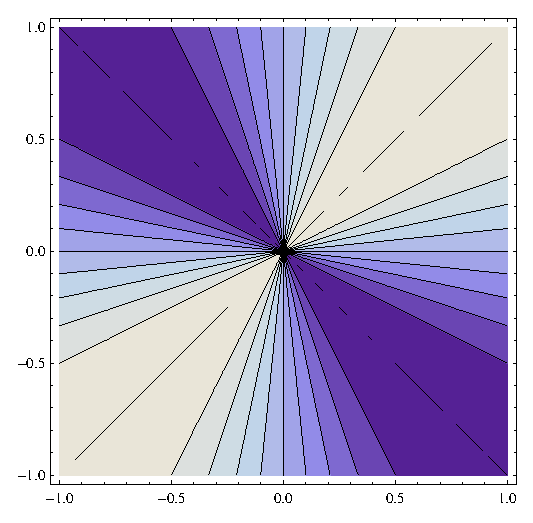
\epsfig{file=fun1cl.eps,clip=,width=4cm,height=4cm}
\vspace{-.7cm}
\end{center}
\caption{Representaci{\'o} gr{\`a}fica de les corbes de nivell de la funci{\'o} $f(x)=\frac{xy}{x^2+y^2}$}
\end{figure}


%\begin{figure}[h!]
%\begin{center}
%\epsfig{file=fun1.eps,clip=,width=4cm,height=4cm}
%\vspace{-.4cm}
%\end{center}
%\caption{Representaci{\'o} gr{\`a}fica de la funci{\'o} $f(x)=\frac{xy}{x^2+y^2}$}
%\end{figure}

\vspace{0.4cm}
\begin{exemple}
Sigui la funci{\'o}
\[
f(x,y)=\begin{cases} \frac{y}{x^2+y} & \text{si $y\not= -x^2$},\\
0 & \text{si $y=-x^2$.}
\end{cases}
\]
Estudiau l'exist{\`e}ncia de $\lim\limits_{(x,y)\to (0,0)} f(x,y)$.
\end{exemple}

\solucio
Calculem primer els l{\'\i}mits segons les rectes $y=mx$.
\begin{align*}
\lim_{(x,y)\to (0,0)\atop y=mx} f(x,y)& =  \lim_{x\to 0} f(x,m x)
= \lim_{x\to 0}\frac{mx}{x^2 + m x} \\ & =  \lim_{x\to 0}
\frac{m}{x + m} = 1.
\end{align*}
no dep{\`e}n de $m$.

Calcularem ara el l{\'\i}mit segons les par{\`a}boles $y=k x^2$ (que passen per
$(0,0)$)

\begin{align*}
\lim_{(x,y)\to (0,0)\atop y=kx^2} f(x,y)& =  \lim_{x\to 0} f(x,k
x^2) = \lim_{x\to 0}\frac{k x^2}{x^2 + k x^2} \\ & =  \lim_{x\to
0} \frac{k}{1 + k} = \frac{k}{1+k}\quad (\mbox{si}\,\, k\not=
-1),
\end{align*}

i, com aquest l{\'\i}mit dep{\`e}n de $k$, aleshores no existeix
$\lim\limits_{(x,y)\to (0,0)} f(x,y)$.


%\begin{figure}[h]
%\begin{center}
%\epsfig{file=f2.eps,clip=,width=6cm,height=6cm}
%\vspace{-.4cm}
%\end{center}
%\caption{Representaci{\'o} gr{\`a}fica de la funci{\'o} $f(x)=\frac{y}{x^2+y}$}
%\end{figure}
%
%\begin{figure}[h]
%\begin{center}
%\epsfig{file=f2cl.eps,clip=,width=6cm,height=6cm}
%\vspace{-.7cm}
%\end{center}
%\caption{Representaci{\'o} gr{\`a}fica de les corbes de nivell de la funci{\'o} $f(x)=\frac{y}{x^2+y}$}
%\end{figure}


%\vspace{0.4cm}
%\begin{exemple}
%Sigui la funci{\'o}
%\[
%f(x,y)=\begin{cases} \frac{x y^2}{x^2+y^4} & \text{si $(x,y)\not=
%(0,0)$},\\ 0 & \text{si $(x,y)=(0,0)$.}
%\end{cases}
%\]
%Estudiau l'exist{\`e}ncia de $\lim\limits_{(x,y)\to (0,0)} f(x,y)$.
%\end{exemple}
%
%\solucio
%Calculem primer els l{\'\i}mits segons les rectes $y=mx$ i segons les par{\`a}boles $y= kx�$.
%\begin{align*}
%\lim_{(x,y)\to (0,0)\atop y=mx} f(x,y)& =  \lim_{x\to 0} f(x,m x)
%= \lim_{x\to 0}\frac{m^2x^3}{x^2 + m^4 x^4} =0, \\
%\lim_{(x,y)\to (0,0)\atop y=kx^2} f(x,y)& =  \lim_{x\to 0} f(x,k
%x^2) = \lim_{x\to 0}\frac{k^2 x^5}{x^2 + k^4 x^8}= 0,
%\end{align*}
%i com podem veure cap dels dos dep{\`e}n del par{\`a}metre.
%
%Calcularem ara el l{\'\i}mit segons les par{\`a}boles $x=k y^2$.
%
%\begin{align*}
%\lim_{(x,y)\to (0,0)\atop x=ky^2} f(x,y)& =  \lim_{y\to 0} f(k
%y^2,y) = \lim_{y\to 0}\frac{k y^2 y^2}{k^2 y^4 + y^4} \\ & =
%\lim_{y\to 0} \frac{k}{1 + k^2} = \frac{k}{1+k^2}.
%\end{align*}
%
%Dep{\`e}n de la par{\`a}bola, aleshores no existeix
%$\lim\limits_{(x,y)\to (0,0)} f(x,y)$.
%\begin{figure}[h]
%\begin{center}
%\epsfig{file=fun3.eps,clip=}
%\vspace{-.4cm}
%\end{center}
%\caption{Representaci{\'o} gr{\`a}fica de la funci{\'o} $f(x)=\frac{xy^2}{x^2+y^4}$}
%\end{figure}
%\begin{figure}[h]
%\begin{center}
%\epsfig{file=fun3cl.eps,clip=,width=6cm,height=6cm}
%\vspace{-.7cm}
%\end{center}
%\caption{Representaci{\'o} gr{\`a}fica de les corbes de nivell de la funci{\'o} $f(x)=\frac{xy^2}{x^2+y^4}$}
%\end{figure}

\vspace{0.4cm}
\subsubsection{C{\`a}lcul de l{\'\i}mits utilitzant les coordenades polars}

El pr{\`o}xim resultat permet fer el c{\`a}lcul d'alguns l{\'\i}mits utilitzant les coordenades polars.


\begin{proposicio}\label{lim coord polars}
Una condici{\'o} necess{\`a}ria i suficient perqu{\`e}:
$$
\lim\limits_{(x,y)\to (0,0)}f(x,y)= a
$$
{\'e}s que
$$
\lim\limits_{r\to 0^+}f(r\,\cos\theta,r\,\sin\theta)= a\qquad\qquad\textrm{per a qualsevol} \ \theta \in [0,2\pi)
$$
\end{proposicio}

\vspace{0.4cm}
\begin{exemple}
Sigui la funci{\'o}
\[
f(x,y)=\begin{cases} \frac{x^2 y}{x^2+y^2} & \text{si $(x,y)\not=
(0,0)$},\\ 0 & \text{si $(x,y)=(0,0)$.}
\end{cases}
\]
Estudiau l'exist{\`e}ncia de $\lim\limits_{(x,y)\to (0,0)} f(x,y)$.
\end{exemple}

\solucio
Es pot veure que el l{\'\i}mits segons, rectes i par{\`a}boles sempre valen $0$. Per{\`o} aix{\`o} no ens permet assegurar que
$\lim\limits_{(x,y)\to (0,0)} f(x,y)=0$. Ara b{\'e} si existeix ha
de ser $0$.

Vegem si $\lim\limits_{(x,y)\to (0,0)} f(x,y)=0$. Ho feim per coordenades polars:

\begin{align*}
\lim\limits_{r\to 0^+}f(r\,\cos\theta,r\,\sin\theta)=&\lim\limits_{r\to 0^+}\frac{r^2\,\cos^2 \theta\;r\,\sin\theta}{r^2\,\cos^2 \theta+r^2\,\sin^2\theta}=\lim\limits_{r\to 0^+}\frac{r^3\,\cos^2 \theta\,\sin\theta}{r^2}\\
&\\
=& \lim\limits_{r\to 0^+}r\,\cos^2 \theta\,\sin\theta=0\qquad \qquad\textrm{per a qualsevol} \ \theta \in [0,2\pi)
\end{align*}

ja que $\ \cos^2 \theta\,\sin\theta\ $ est{\`a} fitat i $r$ tendeix a zero.


Per tant, aplicant la proposici{\'o} \ref{lim coord polars} podem afirmar ara que
$$
\lim\limits_{(x,y)\to (0,0)}
f(x,y)=0
$$


\vspace{0.4cm}
\begin{definicio}[L{\'\i}mits iterats]
$\ $
\noindent Sigui $\ f:\, D\subset \R^2 \longrightarrow \R\ $ i $\ (a,b)\in D\,.$ Siguin $\ C_1, C_2 \ $ entorns de $a$ i $b$ respectivament tals que es puguin considerar les funcions

\hspace{3cm}$\begin{array}{cccc}
p_1: & C_1 & \longrightarrow & \R\\
& x & \longrightarrow & f(x,y)
\end{array}$ \hspace{2cm}$\begin{array}{cccc}
p_2: & C_2 & \longrightarrow & \R\\
& y & \longrightarrow & f(x,y)
\end{array}$

Suposem que existeix la funci{\'o}

\hspace{4cm}$\begin{array}{cccl}
\phi_1: & C_1 & \longrightarrow & \R\\
& x & \longrightarrow & \lim\limits_{y\to b} p_2(y)=\lim\limits_{y\to b} f(x,y)
\end{array}$

Anomenam \textbf{l{\'\i}mit iterat} al l{\'\i}mit
$$\lim\limits_{x\to a} \phi_1(x)=\lim_{x\to
a}\left[ \lim_{y\to b} f(x,y)
\right]$$

De manera an{\`a}loga, l'altre l{\'\i}mit iterat s'obt{\'e} de suposar que existeix la funci{\'o}

\hspace{4cm}$\begin{array}{cccl}
\phi_2: & C_2 & \longrightarrow & \R\\
& y & \longrightarrow & \lim\limits_{x\to a} p_1(x)=\lim\limits_{x\to a} f(x,y)
\end{array}$

i considerar el l{\'\i}mit
$$\lim\limits_{y\to b} \phi_2(y)=\lim_{y\to
b}\left[ \lim_{x\to a} f(x,y)\right]$$
\end{definicio}

\begin{exemple}
Calculau els dos l{\'\i}mits iterats de la funci{\'o} $\ f(x,y)=x^2y+5x y^3+6x\ $ quan $(x,y)\longrightarrow (2,0)\,.$
\end{exemple}

\solucio
$$
\lim_{x\to 2}\left[ \lim_{y\to 0} f(x,y)\right]=\lim_{x\to 2}\left[ \lim_{y\to 0} (x^2y+5x y^3+6x)\right]=\lim_{x\to 2}\left[6x\right]=12
$$

$$
\lim_{y\to 0}\left[\lim_{x\to 2}  f(x,y)\right]=\lim_{y\to 0}\left[\lim_{x\to 2}  (x^2y+5x y^3+6x)\right]=\lim_{y\to 0}\left[4y+10y^3+12\right]=12
$$

\vspace{0.4cm}
\begin{proposicio}
Sigui $\ f:\, D\subset \R^2 \longrightarrow \R\ $ tal que
$\ \lim\limits_{(x,y)\to (a,b)} f(x,y)=l\,. $

a) Suposem  que existeixen
els l{\'\i}mits $\ \lim\limits_{x\to a} f(x,y)\ $ per a tot $y$ d'un entorn de $b$.
Aleshores
\[
\lim_{y\to b}\left[ \lim_{x\to a} f(x,y) \right]= l
\]

b) Suposem  que existeixen
els l{\'\i}mits $\ \lim\limits_{y\to b} f(x,y)\ $ per a tot $x$ d'un entorn de $a$.
Aleshores
\[
\lim_{x\to a}\left[ \lim_{y\to b} f(x,y)\right]= l
\]
\end{proposicio}


\vskip 0.5 cm
\observacio Notem que, si es verifiquen les condicions de la proposici{\'o} i els l{\'\i}mits iterats s{\'o}n distints, aleshores podem afirmar que
no existeix $\lim\limits_{(x,y)\to (a,b)} f(x,y)$.
%Tamb{\'e} podem dir que si
%no existeix qualque l{\'\i}mit iterat, per{\`o} si existeixen els l{\'\i}mits
%$\lim\limits_{x\to a} f(x,y)$ per a tot $y$, i els
%l{\'\i}mits $\lim\limits_{y\to b} f(x,y)$ per a tot $x$, aleshores tampoc existeix
%el  $\lim\limits_{(x,y)\to (a,b)} f(x,y)$.

\vspace{0.4cm}
\begin{exemple}
Considerem la funci{\'o}
\[
f(x,y)=\begin{cases} \frac{x^2- y^2}{x^2+y^2} & \text{si
$(x,y)\not= (0,0)$},\\ 1 & \text{si $(x,y)=(0,0)$.}
\end{cases}
\]
Estudiau l'exist{\`e}ncia de $\lim\limits_{(x,y)\to (0,0)} f(x,y)$.
\end{exemple}

\solucio
Per trobar el l{\'\i}mits iterats, calculam primer els l{\'\i}mits seg{\"u}ents
\begin{align*}
\lim_{x\to 0} f(x,y)&=\lim_{x\to 0} \frac{x^2 -y^2}{x^2+y^2} =
\frac{-y^2}{y^2} = -1 \\
&\\
 \lim_{y\to 0} f(x,y)&=\lim_{y\to 0}
\frac{x^2 -y^2}{x^2+y^2} = \frac{x^2}{x^2} = 1
\end{align*}
Per tant
\begin{align*}
\lim_{y\to 0}\left[\lim_{x\to 0} f(x,y)\right]&=\lim_{y\to 0} -1= -1 \\
 &\\
 \lim_{x\to 0}\left[\lim_{y\to 0}f(x,y)\right]&=\lim_{x\to 0} 1= 1.
\end{align*}
i, com que, els dos l{\'\i}mits iterats s{\'o}n diferents tenim que
no existeix $\lim\limits_{(x,y)\to (0,0)} f(x,y)$.



\subsection{Continu{\"\i}tat}

\begin{definicio}
Sigui $f:\; D\subset \R^n \longrightarrow \R^m$. Direm que $f$
{\'e}s una \textbf{funci{\'o} cont{\'\i}nua en un punt $x_0\in D$} si per a
cada $\ \varepsilon > 0\ $ hi ha un $\ \delta > 0\ $ tal que $\ \| f(x) -
f(x_0) \| < \varepsilon\ $ sempre que $\ x\in D\ $ i $\ \| x - x_0\| <
\delta\,.$
\end{definicio}


\vspace{0.4cm}
\observacions
$\ $

1.- Si $x_0$ {\'e}s un \textbf{punt a{\"\i}llat} de $\ D\ $, (aix{\`o} vol dir que existeix un
$\ \varepsilon > 0\ $ tal que

 $\ B(x_0,\varepsilon)\cap D =\{x_0 \}$), aleshores qualsevol funci{\'o} {\'e}s
cont{\'\i}nua  en $x_0$.

\vspace{0.3cm}
2.- Si $x_0$ {\'e}s un punt d'acumulaci{\'o} de $D$, dir que $f$ {\'e}s cont{\'\i}nua en $x_0$
equival a dir que $\ \lim\limits_{x\to x_0} f(x) = f(x_0)$.

\vspace{0.4cm}
\begin{exemple}
Considerem ara algunes de les funcions estudiades als exemples de
la subsecci{\'o} anterior.
\end{exemple}

\begin{itemize}
  \item[1.-] Les funcions
  \[
f(x,y)=\begin{cases} \frac{xy}{x^2+y^2} & \text{si $(x,y)\not=
(0,0)$}\\ 0 & \text{si $(x,y)=(0,0)$} \end{cases} \qquad
\mbox{i}\qquad g(x,y)=\begin{cases} \frac{y}{x^2+y} & \text{si
$y\not= -x^2$}\\ 0 & \text{si $y=-x^2$}\end{cases}
  \]

  no s{\'o}n cont{\'\i}nues en $(0,0)$ ja que hem vist que no
  existeixen els l{\'\i}mits $\ \lim\limits_{(x,y)\to (0,0)} f(x,y)\ $
  i $\ \lim\limits_{(x,y)\to (0,0)} g(x,y)$.

  \item[2.-] La funci{\'o}
$$
f(x,y)=\begin{cases} \frac{x^2 y}{x^2+y^2} & \text{si $(x,y)\not=
(0,0)$}\\ 0 & \text{si $(x,y)=(0,0)$}
\end{cases}$$


{\'e}s cont{\'\i}nua en $(0,0)$ ja que hem comprovat que\\

 \hspace{2cm}$\ \lim\limits_{(x,y)\to (0,0)} f(x,y)=0=f(0,0)$
\end{itemize}


%\vspace{0.4cm}
%\observacio Si la funci{\'o} $f(x,y)$ {\'e}s cont{\'\i}nua en $(0,0)$, aleshores es
%veu que en la representaci{\'o} gr{\`a}fica de les corbes de nivell t{\'e} el mateix color en
%un entorn del punt $(0,0)$. En canvi, si $f(x,y)$ no {\'e}s cont{\'\i}nua, per qualsevol
%entorn que agafem devora $(0,0)$,  per molt petit que sigui, sempre hi ha distints
%colors. Veure la gr{\`a}fica de la funci{\'o} $f(x,y)=\frac{xy}{x^2+y^2}$ com exemple de
%funci{\'o} discont{\'\i}nua i la gr{\`a}fica de la funci{\'o} $f(x,y)=\frac{x^2y}{x^2+y^2}$
%com exemple de  funci{\'o} cont{\'\i}nua.

\vspace{0.4cm}
\begin{definicio}
Sigui $f:\; D\subset \R^n \longrightarrow \R$. Direm que $f$ {\'e}s una funci{\'o}
\textbf{cont{\'\i}nua en $D$} si {\'e}s cont{\'\i}nua en cada punt de $D$.
\end{definicio}

\vspace{0.4cm}
\observacio Les propietats elementals de les funcions cont{\'\i}nues d'una variable real tenen versions corresponents per les funcions de diverses variables. Aix{\'\i}, la suma, producte, quocient
(quan est{\`a} ben definit) de funcions cont{\'\i}nues s{\'o}n tamb{\'e} cont{\'\i}nues, com
tamb{\'e} ho {\'e}s la composici{\'o} de funcions cont{\'\i}nues.

\vspace{0.4cm}
\begin{teorema}
Siguin $\ f,g : D\subset\R^n\,\longrightarrow\,\R^m\ $ i $\ c\in\R$.
Aleshores,
\begin{itemize}
  \item[(i)] Si $f$ {\'e}s cont{\'\i}nua en $x_0$ aleshores, la
  funci{\'o} $c\, f : D\subset\R^n\,\longrightarrow\,\R^m$
  donada per $(cf)(x) = c\, f(x)$ {\'e}s cont{\'\i}nua en
  $x_0$.
  \item[(ii)] Si $f$ i $g$ s{\'o}n funcions cont{\'\i}nues en $x_0$
  aleshores, la funci{\'o} $f+g \, :\,
  D\subset\R^n\,\longrightarrow\,\R^m$ donada per
  $(f+g)(x)=f(x)+g(x)$ {\'e}s cont{\'\i}nua en $x_0$.
  \item[(iii)] Si $m=1$ i  $f$, $g$ s{\'o}n funcions cont{\'\i}nues en $x_0$
  aleshores, la funci{\'o} $f\, g:
  D\subset\R^n\longrightarrow\R$ donada per
  $(f \cdot g)(x)=f(x)\cdot g(x)$ {\'e}s cont{\'\i}nua en $x_0$.
  \item[(iv)] Si $m=1$ i $f$ {\'e}s una funci{\'o} no cont{\'\i}nua nul.la en
  $x_0$ aleshores, la funci{\'o} \\

  $\qquad \displaystyle\frac{1}{f}:
  D\subset\R^n\,\longrightarrow\,\R\ $ donada per
  $\ \left(\displaystyle \frac{1}{f}\right) (x)=\displaystyle\frac{1}{f(x)}$ {\'e}s cont{\'\i}nua en $x_0$.
\end{itemize}
\end{teorema}

\vspace{0.3cm}
Com a conseq{\"u}{\`e}ncia immediata dels dos primers apartats del teorema anterior tenim el seg{\"u}ent resultat.

\vspace{0.4cm}
\begin{teorema}
Tota funci{\'o} lineal $\ f:\R^n \longrightarrow\R^m\ $ {\'e}s una
funci{\'o} cont{\'\i}nua.
\end{teorema}

\vspace{0.3cm}
La relaci{\'o} entre la continu{\"\i}tat d'una funci{\'o} vectorial i
la continu{\"\i}tat de les seves funcions coordenades ve donada pel seg{\"u}ent resultat.

\vspace{0.4cm}
\begin{proposicio}
Sigui $f:\; D\subset \R^n \longrightarrow \R^m$, $f=(f_1,f_2,\ldots ,f_m)$ i $x_0\in D$.
Aleshores $f$  {\'e}s cont{\'\i}nua en $x_0$ si, i nom{\'e}s si, $f_i$  {\'e}s cont{\'\i}nua en $x_0$
per a tot $i=1,\ldots , m$.
\end{proposicio}




\vspace{0.3cm}
El seg{\"u}ent teorema que ens dona la continu{\"\i}tat de la composici{\'o} de funcions.

\vspace{0.4cm}
\begin{teorema}
Siguin  $\ f:D\subset \R^n \longrightarrow \R^m\,,\ g:B\subset \R^m \longrightarrow \R^p\ $ tals que $\ f(D)\subset B\,. $ Si $f$ {\'e}s
cont{\'\i}nua en $a\in D$ i $g$ {\'e}s cont{\'\i}nua en
$b=f(a)$ aleshores, $g\circ f$ {\'e}s cont{\'\i}nua en $a$.
\end{teorema}



\vspace{0.4cm}
\observacio Aquest darrer teorema, al igual que en el cas de
funcions reals de variable real, ens permet deduir la
continu{\"\i}tat de moltes funcions de diverses variables.


\vspace{0.4cm}
\exemples
\begin{itemize}
  \item[1.-] Sigui $\ f:\R^2\longrightarrow\R\ $ definida per $\ f(x,y)=\sin (x^2y)\,. $

  El domini de $f$ {\'e}s $\ \R^2\ $ i si consideram les funcions
  $\ g:\R^2\longrightarrow\R\,,\ \  h:\R\longrightarrow\R\ $ donades per $\ g(x,y)= x^2 y\ $  i
  $\ h(z)=\sin z\ $ aleshores  $\ f=h\circ g\,.$

Com que $g$ {\'e}s cont{\'\i}nua en tot $\R^2$ i $h$ {\'e}s
  una funci{\'o} cont{\'\i}nua en tot $\R$ tenim que, $f$ {\'e}s
  cont{\'\i}nua en tot $\R^2\,.$

\vspace{0.3cm}
  \item[2.-] Sigui $\ f:\R^2\longrightarrow\R\ $ definida per $\ f(x,y)=\ln (x^2+y^2)\,. $

  El domini de $f$ {\'e}s $\ D=\R^2\setminus\{ (0,0) \}\ $ i si consideram les funcions
  $\ g:\R^2\longrightarrow\R\,,$

  $h:\R^+\setminus\{0 \}\longrightarrow\R\ $ donades per $\ g(x,y)= x^2 +y^2\ $  i
  $\ h(z)=\ln z\ $ verifiquen que   $\ g(D)\subset \R^+\setminus\{0 \}\,, $ aleshores$\ f=h\circ g\,.$

Com que $g$ {\'e}s cont{\'\i}nua en tot $\R^2$ i $h$ {\'e}s
  una funci{\'o} cont{\'\i}nua en $\R^+\setminus \{ 0\}$ tenim que, $f$ {\'e}s
  cont{\'\i}nua en $\R^2\setminus\{ (0,0) \}\,.$



\vspace{0.3cm}
  \item[3.-] Sigui $\ f:\R^2\longrightarrow\R\ $ definida per $\ f(x,y)=\displaystyle\frac{e^{x+y}}{x+y}\,. $

  El domini de $f$ {\'e}s
  $$D=\R^2\setminus\{(x,y)\in\R^2\ :\  x+y=0 \}$$
   i si consideram les funcions
  $\ g:\R^2\longrightarrow\R\,,\ \ h:\R\setminus\{0 \}\longrightarrow\R\ $ donades per $\ g(x,y)=x +y\ $  i
  $\ h(z)=\frac{e^z}{z}\ $ verifiquen que   $\ g(D)\subset \R\setminus\{0 \}\,, $ aleshores$\ f=h\circ g\,.$

Com que $g$ {\'e}s cont{\'\i}nua en tot $\R^2$ i $h$ {\'e}s
  una funci{\'o} cont{\'\i}nua en $\R\setminus \{ 0\}$ tenim que, $f$ {\'e}s
  cont{\'\i}nua en $D\,.$


\vspace{0.3cm}
  \item[4.-] Sigui $\ f:\R^2\longrightarrow\R\ $ definida per $\ f(x,y)=\ln (\cos (x^2+y^2))\,. $

  El domini de $f$ {\'e}s
  $$D=\{ (x,y)\in\R^2\ :\ -\frac{\pi}{2}+2\pi n < x^2 +y^2 <
  \frac{\pi}{2}+2\pi n\,,\ \ n\in\Z\}$$
   i si consideram les funcions
  $\ g:\R^2\longrightarrow\R\,,\ \ h:\R\longrightarrow\R\ \,,\ \ k:\R^+\longrightarrow\R\ $ donades per $\ g(x,y)=x^2+y^2\,, \ h(z)=\cos z\ $  i
  $\ k(u)=\ln u\ $ verifiquen que   $\ h(g(D))\subset \R^+\,, $ aleshores$\ f=k\circ h\circ g\,.$

Com que $g$ {\'e}s cont{\'\i}nua en tot $\R^2\,, $  $h$ {\'e}s
  cont{\'\i}nua en tot $\ \R$ i $k$ {\'e}s cont{\'\i}nua en $\ \R^+\ $ tenim que, $f$ {\'e}s
  cont{\'\i}nua en $\ D\,.$

  \end{itemize}



Per acabar donam un resultat que ja ten{\'\i}em per funcions d'una variable.


\vspace{0.4cm}
\begin{teorema}[Teorema de Weierstrass]
Si $f:D\subset \R^n \longrightarrow \R$ {\'e}s cont{\'\i}nua i $D$ {\'e}s compacte,
aleshores $f$ {\'e}s fitada i t{\'e} un m{\`a}xim i un m{\'\i}nim en $D$.
\end{teorema}



\end{document}
